% !TEX TS-program = pdflatex
% !TEX encoding = UTF-8 Unicode

% This is a simple template for a LaTeX document using the "article" class.
% See "book", "report", "letter" for other types of document.

\documentclass[11pt]{article} % use larger type; default would be 10pt

\usepackage[utf8]{inputenc} % set input encoding (not needed with XeLaTeX)

%%% Examples of Article customizations
% These packages are optional, depending whether you want the features they provide.
% See the LaTeX Companion or other references for full information.

%%% PAGE DIMENSIONS
\usepackage{geometry} % to change the page dimensions
\geometry{a4paper} % or letterpaper (US) or a5paper or....
% \geometry{margin=2in} % for example, change the margins to 2 inches all round
% \geometry{landscape} % set up the page for landscape
%   read geometry.pdf for detailed page layout information

\usepackage{graphicx} % support the \includegraphics command and options

% \usepackage[parfill]{parskip} % Activate to begin paragraphs with an empty line rather than an indent

%%% PACKAGES
\usepackage{graphicx}
\usepackage{listings}
\usepackage{booktabs} % for much better looking tables
\usepackage{array} % for better arrays (eg matrices) in maths
\usepackage{paralist} % very flexible & customisable lists (eg. enumerate/itemize, etc.)
\usepackage{verbatim} % adds environment for commenting out blocks of text & for better verbatim
\usepackage{subfig} % make it possible to include more than one captioned figure/table in a single float
% These packages are all incorporated in the memoir class to one degree or another...

%%% HEADERS & FOOTERS
\usepackage{fancyhdr} % This should be set AFTER setting up the page geometry
\pagestyle{fancy} % options: empty , plain , fancy
\renewcommand{\headrulewidth}{0pt} % customise the layout...
\lhead{}\chead{}\rhead{}
\lfoot{}\cfoot{\thepage}\rfoot{}

%%% SECTION TITLE APPEARANCE
\usepackage{sectsty}
\allsectionsfont{\sffamily\mdseries\upshape} % (See the fntguide.pdf for font help)
% (This matches ConTeXt defaults)

%%% ToC (table of contents) APPEARANCE
\usepackage[nottoc,notlof,notlot]{tocbibind} % Put the bibliography in the ToC
\usepackage[titles,subfigure]{tocloft} % Alter the style of the Table of Contents
\renewcommand{\cftsecfont}{\rmfamily\mdseries\upshape}
\renewcommand{\cftsecpagefont}{\rmfamily\mdseries\upshape} % No bold!

%%% END Article customizations

%%% The "real" document content comes below...

\title{Concurrent Programming CW1 - Museum}
\author{Thomas Taylor-Hall}
%\date{} % Activate to display a given date or no date (if empty),
         % otherwise the current date is printed 

\begin{document}
\maketitle

%QUESTION 1
\section{Structure Diagram}

\begin{figure}[h!]
	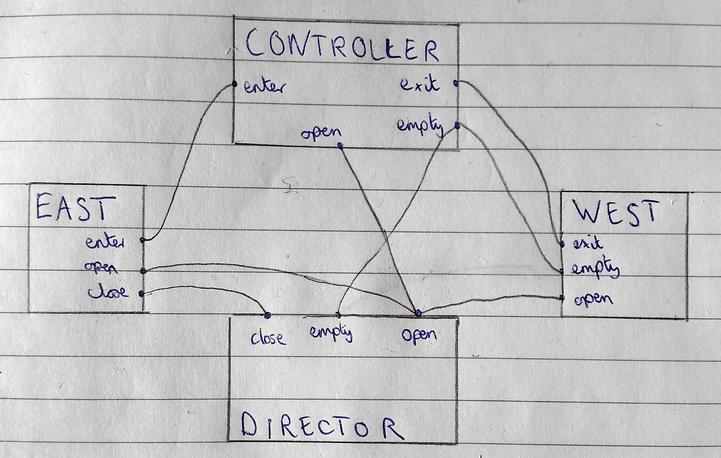
\includegraphics[width=\textwidth]{structure-diagram.jpg}
	\caption{Structure diagram showing the relationships between the processes in the museum model.}
\end{figure}


\pagebreak
%QUESTION 2
\section{Finite State Process Model}

\lstinputlisting[language=Java]{museum.lts}

The entrance and exit jump between open and closed states. The entrance is open when the museum is not yet full, and closed on
the director's signal. The exit is always open except when the museum is empty, as no-one can exit an empty museum. The controller is
initialized by opening the museum with no visitors inside, and permits entrances and exits depending on the number of visitors. The
four processes are composed to form the \textbf{$||$MUSEUM} process.


\pagebreak
%QUESTION 3 TODO: not sure about this!
\section{Test Process}

\begin{lstlisting}[language=Java]
TEST = (open -> close -> TEST |
	      close -> enter  -> ERROR).

||MUSEUM_TEST = (MUSEUM || TEST).
\end{lstlisting}

This \textbf{TEST} process synchronizes with the museum on \textit{open}, \textit{close} and \textit{enter}. It tests whether a visitor can enter the museum after closing time. LTSA shows no deadlocks or process violations meaning that the museum system passes this test.



\pagebreak
%QUESTION 4
\section{Safety Trace}
If we compose the \textbf{MUSEUM} system with the following process \textbf{P},

\begin{lstlisting}[language=Java]
P = STOP + {exit}.
\end{lstlisting}

then the action \textit{exit} can never happen, as we need to arrive at the \textbf{STOP} state before. This means we can hit a potential deadlock in our system, whenever the museum is closed by the director with any amount of visitors in it. The safety menu in LTSA gives the following trace leading to deadlock:

\begin{lstlisting}[language=Java]
(open -> enter -> close )
\end{lstlisting}

After closing, we cannot perform \textit{exit} without process \textbf{P} being synchronised, leading to the \textbf{STOP} state. Hence the visitor that has entered the museum cannot leave, and the museum will remain closed forever, as we cannot perform the \textit{empty} action.



\end{document}
